\documentclass[tikz]{standalone}
\usepackage{siunitx}

\begin{document}
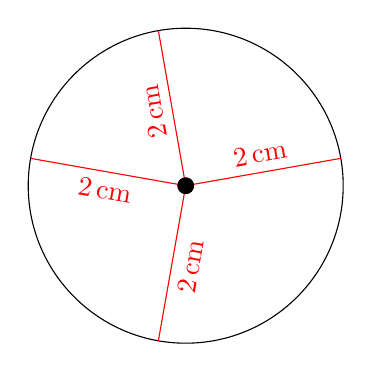
\begin{tikzpicture}
    \draw (0,0) circle (2);
    \draw[red] (0,0) -- node[midway,rotate=10,above] {$\qty{2}{\centi\metre}$} ({2*cos(10)},{2*sin(10});
    \draw[red] (0,0) -- node[midway,rotate=100,above] {$\qty{2}{\centi\metre}$} ({2*cos(100)},{2*sin(100});
    \draw[red] (0,0) -- node[midway,rotate=-10,below] {$\qty{2}{\centi\metre}$} ({2*cos(170)},{2*sin(170});
    \draw[red] (0,0) -- node[midway,rotate=80,below] {$\qty{2}{\centi\metre}$} ({2*cos(260)},{2*sin(260});
    \draw[black,fill=black] (0,0) circle (0.1);
\end{tikzpicture}
\end{document}